\documentclass[12pt]{article}\usepackage[]{graphicx}\usepackage[]{color}
%% maxwidth is the original width if it is less than linewidth
%% otherwise use linewidth (to make sure the graphics do not exceed the margin)
\makeatletter
\def\maxwidth{ %
  \ifdim\Gin@nat@width>\linewidth
    \linewidth
  \else
    \Gin@nat@width
  \fi
}
\makeatother

\definecolor{fgcolor}{rgb}{0.345, 0.345, 0.345}
\newcommand{\hlnum}[1]{\textcolor[rgb]{0.686,0.059,0.569}{#1}}%
\newcommand{\hlstr}[1]{\textcolor[rgb]{0.192,0.494,0.8}{#1}}%
\newcommand{\hlcom}[1]{\textcolor[rgb]{0.678,0.584,0.686}{\textit{#1}}}%
\newcommand{\hlopt}[1]{\textcolor[rgb]{0,0,0}{#1}}%
\newcommand{\hlstd}[1]{\textcolor[rgb]{0.345,0.345,0.345}{#1}}%
\newcommand{\hlkwa}[1]{\textcolor[rgb]{0.161,0.373,0.58}{\textbf{#1}}}%
\newcommand{\hlkwb}[1]{\textcolor[rgb]{0.69,0.353,0.396}{#1}}%
\newcommand{\hlkwc}[1]{\textcolor[rgb]{0.333,0.667,0.333}{#1}}%
\newcommand{\hlkwd}[1]{\textcolor[rgb]{0.737,0.353,0.396}{\textbf{#1}}}%
\let\hlipl\hlkwb

\usepackage{framed}
\makeatletter
\newenvironment{kframe}{%
 \def\at@end@of@kframe{}%
 \ifinner\ifhmode%
  \def\at@end@of@kframe{\end{minipage}}%
  \begin{minipage}{\columnwidth}%
 \fi\fi%
 \def\FrameCommand##1{\hskip\@totalleftmargin \hskip-\fboxsep
 \colorbox{shadecolor}{##1}\hskip-\fboxsep
     % There is no \\@totalrightmargin, so:
     \hskip-\linewidth \hskip-\@totalleftmargin \hskip\columnwidth}%
 \MakeFramed {\advance\hsize-\width
   \@totalleftmargin\z@ \linewidth\hsize
   \@setminipage}}%
 {\par\unskip\endMakeFramed%
 \at@end@of@kframe}
\makeatother

\definecolor{shadecolor}{rgb}{.97, .97, .97}
\definecolor{messagecolor}{rgb}{0, 0, 0}
\definecolor{warningcolor}{rgb}{1, 0, 1}
\definecolor{errorcolor}{rgb}{1, 0, 0}
\newenvironment{knitrout}{}{} % an empty environment to be redefined in TeX

\usepackage{alltt}

%\usepackage{times}
\usepackage{hyperref}
\hypersetup{pdfpagemode=UseNone} % don't show bookmarks on initial view
\hypersetup{colorlinks, urlcolor={blue}}

% revise margins
\setlength{\headheight}{0.0in}
\setlength{\topmargin}{0.0in}
\setlength{\headsep}{0.0in}
\setlength{\textheight}{8.65in}
\setlength{\footskip}{0.35in}
\setlength{\oddsidemargin}{0.0in}
\setlength{\evensidemargin}{0.0in}
\setlength{\textwidth}{6.5in}

\setlength{\parskip}{6pt}
\setlength{\parindent}{0pt}
\IfFileExists{upquote.sty}{\usepackage{upquote}}{}
\begin{document}

%\sffamily
{\textbf{EPDS Survey}}

%\href{http://kbroman.org}{Karl W Broman}
Alejandra Benitez and the Preterm Birth Initiative

%This is a portion of the ``\href{http://www.rqtl.org/rqtltour2.pdf}{A shorter tour of R/qtl}''
%tutorial, developed here in multiple formats to illustrate the use of knitr.
%This particular document is written with \href{http://www.latex-project.org}{LaTeX}.



\bigskip
%\sffamily 
\textbf{Abstract}
\newline
%\nopagebreak

\textit{Results}
Our preliminary results 

\textit{Conclusions}


\section{Results}
\begin{itemize}
\item Table 1 for population, age, SES, region
\end{itemize}
%
%\textbf{Results}
%
You then load the R/qtl package using the {\tt library} function:

%<<load_qtl>>=
%library(qtl)
%@





\begin{knitrout}
\definecolor{shadecolor}{rgb}{0.969, 0.969, 0.969}\color{fgcolor}\begin{kframe}
\begin{alltt}
\hlstd{dat} \hlkwb{=} \hlkwd{read.csv}\hlstd{(}\hlkwd{here}\hlstd{(}\hlstr{"data"}\hlstd{,} \hlstr{"epds_Data.csv"}\hlstd{))}
\hlstd{ctrl_n} \hlkwb{=} \hlstd{dat}\hlopt{$}\hlstd{Number.of.Observations.Postpartum[dat}\hlopt{$}\hlstd{Arm} \hlopt{==} \hlstr{"Control"} \hlopt{|} \hlstd{dat}\hlopt{$}\hlstd{Arm} \hlopt{==} \hlstr{"Control "}\hlstd{]}
\hlstd{ctrl_n} \hlkwb{=} \hlstd{ctrl_n[ctrl_n} \hlopt{>} \hlnum{11}\hlstd{]}
\hlkwd{length}\hlstd{(ctrl_n)}
\end{alltt}
\begin{verbatim}
## [1] 14
\end{verbatim}
\begin{alltt}
\hlstd{interv_n} \hlkwb{=} \hlstd{dat}\hlopt{$}\hlstd{Number.of.Observations.Postpartum[dat}\hlopt{$}\hlstd{Arm} \hlopt{==} \hlstr{"Group"} \hlopt{|} \hlstd{dat}\hlopt{$}\hlstd{Arm} \hlopt{==} \hlstr{"Group "}\hlstd{]}
\hlstd{interv_n} \hlkwb{=} \hlstd{interv_n[interv_n} \hlopt{>} \hlnum{11}\hlstd{]}
\hlkwd{length}\hlstd{(interv_n)}
\end{alltt}
\begin{verbatim}
## [1] 14
\end{verbatim}
\begin{alltt}
\hlstd{current.rates} \hlkwb{=} \hlkwd{c}\hlstd{(ctrl_n, interv_n)}

\hlstd{ctrl_rt} \hlkwb{=} \hlstd{dat}\hlopt{$}\hlstd{Postpartum.Depression.Prevalence[(dat}\hlopt{$}\hlstd{Arm} \hlopt{==} \hlstr{"Control"} \hlopt{|} \hlstd{dat}\hlopt{$}\hlstd{Arm} \hlopt{==} \hlstr{"Control "}\hlstd{)} \hlopt{&}
                                                 \hlstd{dat}\hlopt{$}\hlstd{Number.of.Observations.Postpartum} \hlopt{>} \hlnum{11}\hlstd{]}
\hlkwd{mean}\hlstd{(ctrl_rt)}
\end{alltt}
\begin{verbatim}
## [1] 0.1100286
\end{verbatim}
\begin{alltt}
\hlstd{interv_rt} \hlkwb{=} \hlstd{dat}\hlopt{$}\hlstd{Postpartum.Depression.Prevalence[(dat}\hlopt{$}\hlstd{Arm} \hlopt{==} \hlstr{"Group"} \hlopt{|} \hlstd{dat}\hlopt{$}\hlstd{Arm} \hlopt{==} \hlstr{"Group "}\hlstd{)} \hlopt{&}
                                                   \hlstd{dat}\hlopt{$}\hlstd{Number.of.Observations.Postpartum} \hlopt{>} \hlnum{11}\hlstd{]}
\hlkwd{mean}\hlstd{(interv_rt)}
\end{alltt}
\begin{verbatim}
## [1] 0.03764286
\end{verbatim}
\end{kframe}
\end{knitrout}


\begin{knitrout}
\definecolor{shadecolor}{rgb}{0.969, 0.969, 0.969}\color{fgcolor}
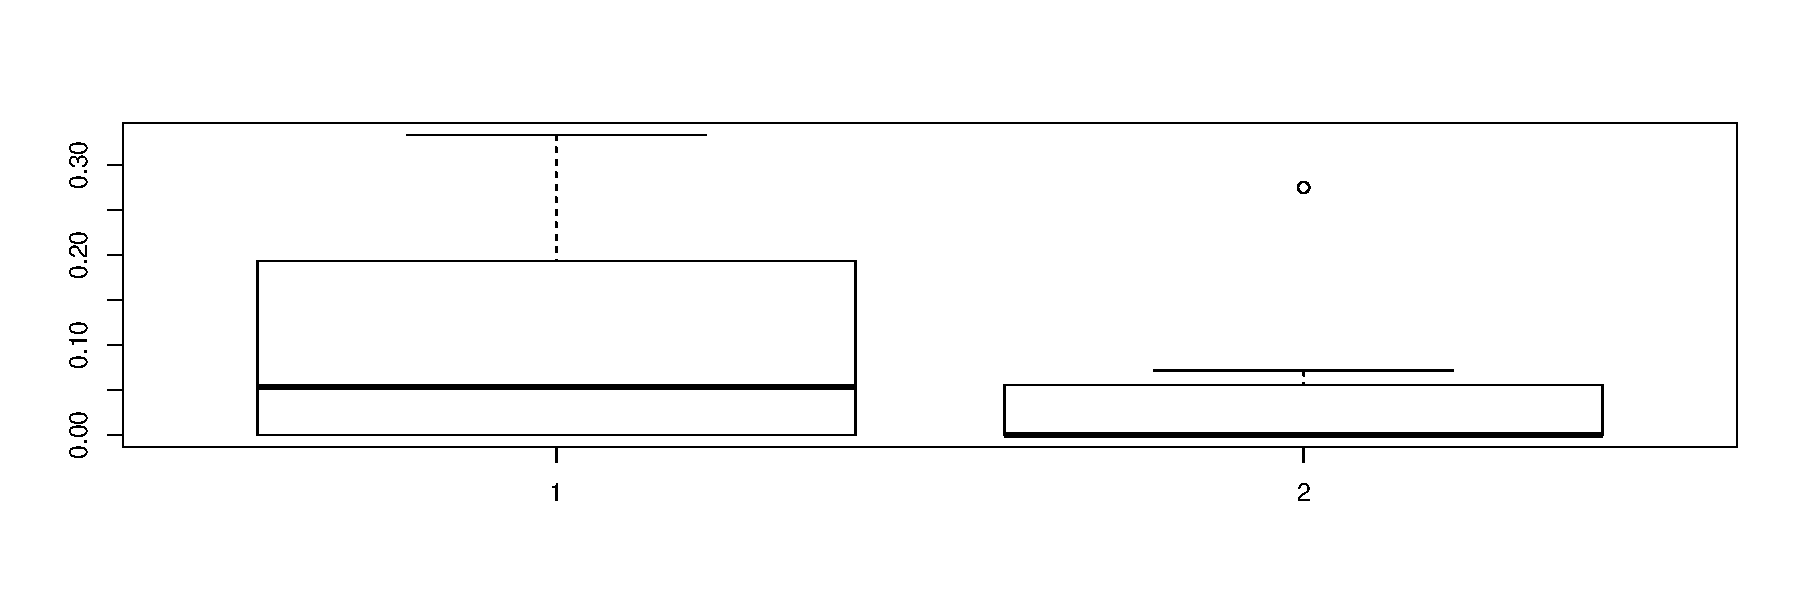
\includegraphics[width=4in,height=4in]{RnwFigs/inclusion_criteria-1} 

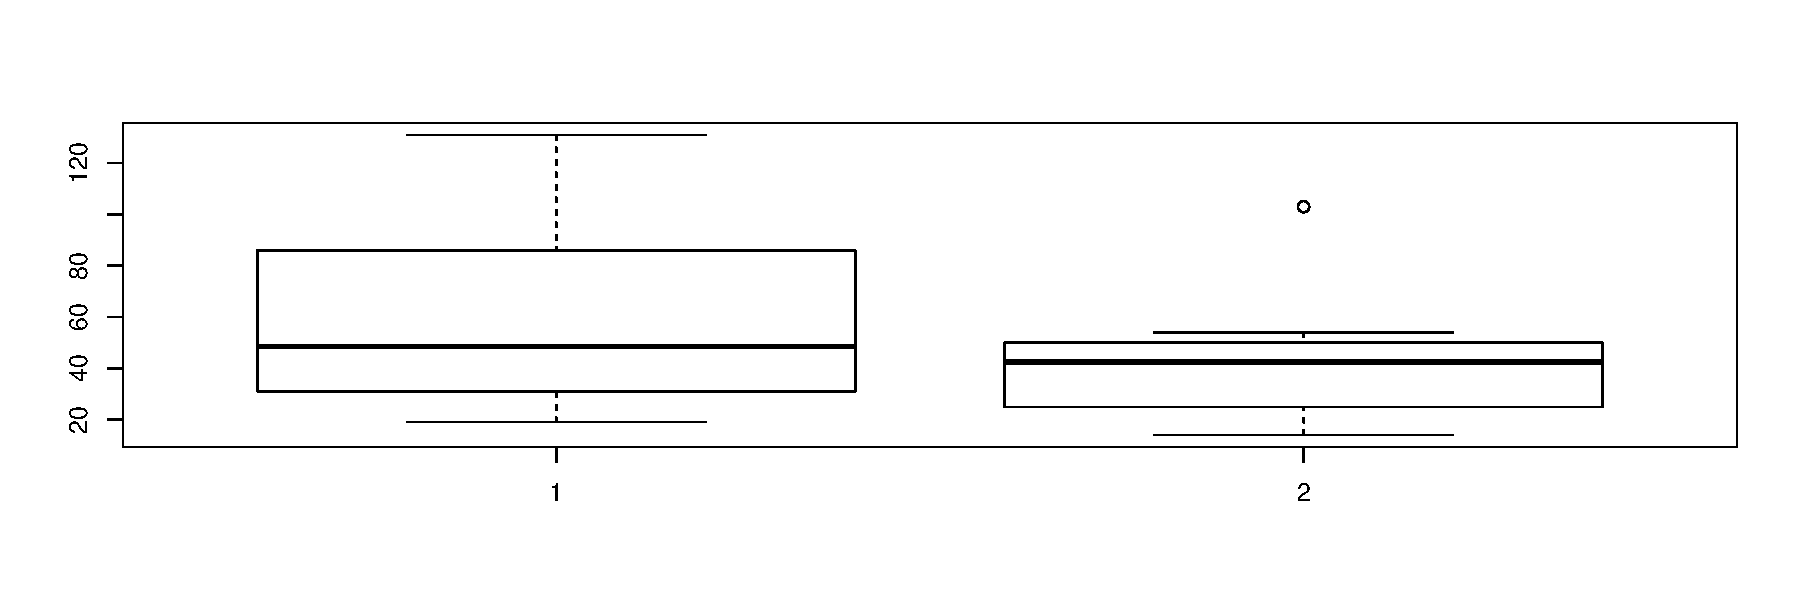
\includegraphics[width=4in,height=4in]{RnwFigs/inclusion_criteria-2} 

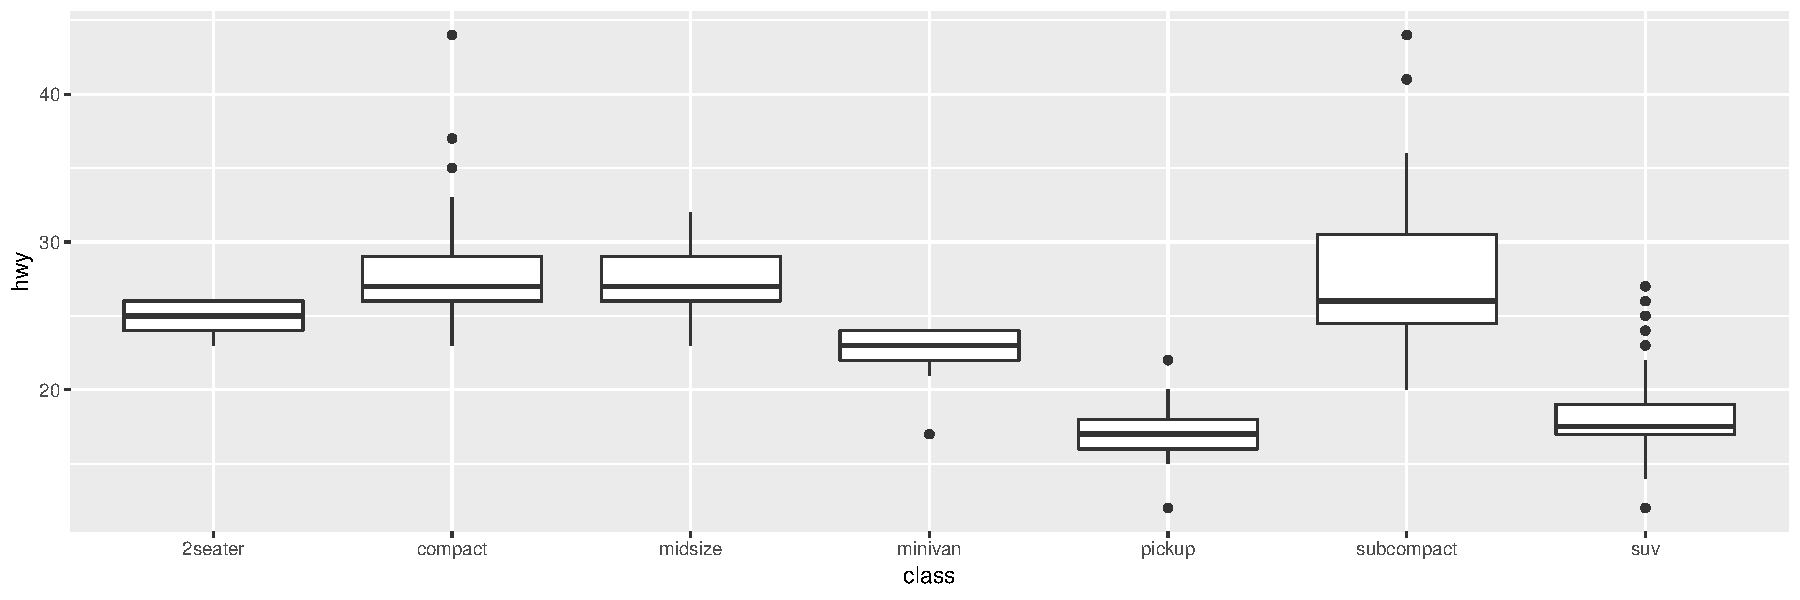
\includegraphics[width=4in,height=4in]{RnwFigs/inclusion_criteria-3} 

\end{knitrout}





\bigskip
{\sffamily \textbf{R and package versions used}}
\nopagebreak




\begin{knitrout}
\definecolor{shadecolor}{rgb}{0.969, 0.969, 0.969}\color{fgcolor}\begin{kframe}
\begin{alltt}
\hlkwd{sessionInfo}\hlstd{()}
\end{alltt}
\begin{verbatim}
## R version 3.5.0 (2018-04-23)
## Platform: x86_64-apple-darwin15.6.0 (64-bit)
## Running under: macOS High Sierra 10.13.1
## 
## Matrix products: default
## BLAS: /Library/Frameworks/R.framework/Versions/3.5/Resources/lib/libRblas.0.dylib
## LAPACK: /Library/Frameworks/R.framework/Versions/3.5/Resources/lib/libRlapack.dylib
## 
## locale:
## [1] en_US.UTF-8/en_US.UTF-8/en_US.UTF-8/C/en_US.UTF-8/en_US.UTF-8
## 
## attached base packages:
## [1] stats     graphics  grDevices utils     datasets 
## [6] methods   base     
## 
## other attached packages:
## [1] ggplot2_3.1.1   qtl_1.42-8      parsedate_1.1.3
## [4] geepack_1.2-1   dplyr_0.8.0.1   here_0.1       
## [7] knitr_1.22     
## 
## loaded via a namespace (and not attached):
##  [1] Rcpp_1.0.1       rstudioapi_0.10  magrittr_1.5    
##  [4] munsell_0.5.0    tidyselect_0.2.5 colorspace_1.4-1
##  [7] R6_2.4.0         rlang_0.3.4      plyr_1.8.4      
## [10] stringr_1.4.0    highr_0.7        tools_3.5.0     
## [13] grid_3.5.0       parallel_3.5.0   gtable_0.3.0    
## [16] xfun_0.5         withr_2.1.2      lazyeval_0.2.2  
## [19] assertthat_0.2.1 rprojroot_1.3-2  tibble_2.1.1    
## [22] crayon_1.3.4     purrr_0.3.2      glue_1.3.1      
## [25] evaluate_0.13    labeling_0.3     stringi_1.3.1   
## [28] compiler_3.5.0   pillar_1.3.1     scales_1.0.0    
## [31] backports_1.1.4  pkgconfig_2.0.2
\end{verbatim}
\end{kframe}
\end{knitrout}

% \bibliography{ga_pred} 
% \bibliographystyle{ieeetr}

\end{document}
